\section{Results at 8 bits per creature}\label{sec:main8}

This is the stage that decides the claim: \N{runs.main8} of \N{expected.main8} counted runs
(4 numbers of creatures, 5 body widths, 2 kinds of word use, 5 repeats), \N{steps.main8} steps of
training each. \N{missing.main8} runs are missing.

\subsection{Facts known}

\begin{figure}[H]
\centering
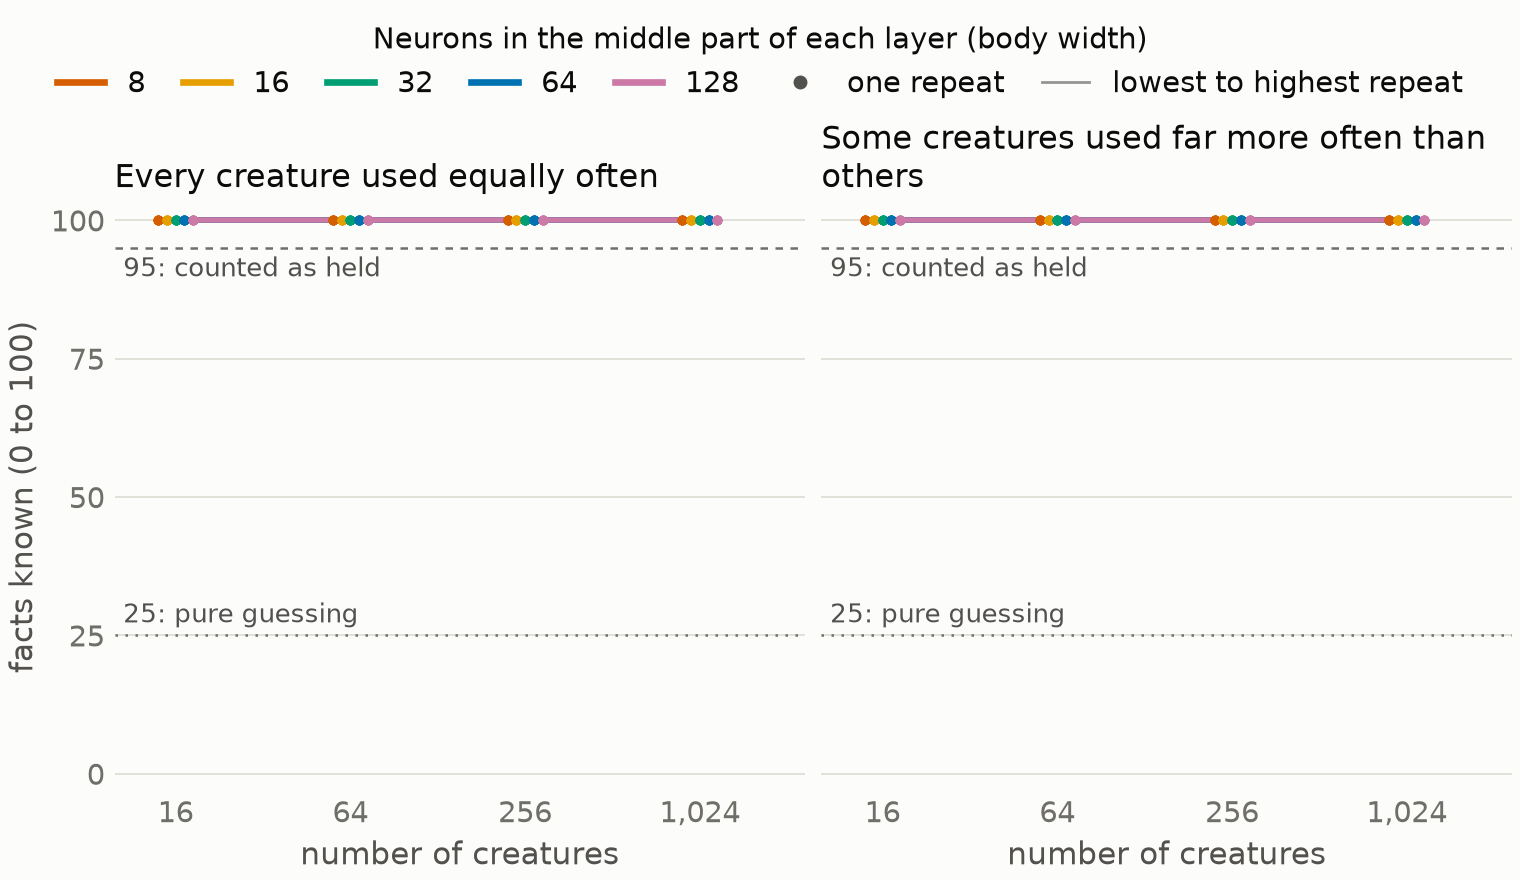
\includegraphics[width=0.68\textwidth]{figures/fig1_main.png}
\caption{Facts known at 8 bits per creature, by number of creatures and body width.}\label{fig:main}
\end{figure}

\reads{fig:main} The left panel is equal use, the right panel unequal use. Along the bottom is the
number of creatures. Up the side is facts known: 100 is every fact right, 25 is pure guessing, and
the dashed line at \N{rule.held} is the line the plan called ``held''. Each colour is one body
width, and each dot is one of the \N{rule.repeats} repeats.

\shows{fig:main} Every dot sits on 100. The five colours lie on top of each other, so only the top
one can be seen. The lowest score of any run was \N{main8.facts.lowest} and the highest
\N{main8.facts.highest}. With 1,024 creatures and the smallest body (width 8, with
\N{main8.c16.b8.equal.params.middle} trained numbers in the middle parts) the facts were as well
known as with 16 creatures.

\textbf{The predictions and the verdict.} Worked out by the rule of section \ref{sec:rule}:

\begin{center}\small
\begin{tabularx}{\textwidth}{@{}>{\raggedright\arraybackslash}p{0.34\textwidth}>{\raggedright\arraybackslash}XX@{}}
\toprule
 & Equal use & Unequal use\\
\midrule
P1: with 16 creatures every body width reaches \N{rule.held} & \N{p1.equal.result} & \N{p1.zipf.result}\\
P2: at width 8, 1,024 creatures are \N{rule.gap} or more points below 16 creatures
  & \N{p2.equal.result} (median gap \N{p2.equal.gap} points) & \N{p2.zipf.result} (median gap \N{p2.zipf.gap})\\
P3: on 1,024 creatures, width 128 is \N{rule.gap} or more points above width 8
  & \N{p3.equal.result} (median gap \N{p3.equal.gap}) & \N{p3.zipf.result} (median gap \N{p3.zipf.gap})\\
P4: at every width, 1,024 creatures are within \N{rule.gap} points of 16 creatures
  & \N{p4.equal.result} & \N{p4.zipf.result}\\
\midrule
\textbf{Verdict on the claim} & \textbf{\N{verdict.equal}} & \textbf{\N{verdict.zipf}}\\
\bottomrule
\end{tabularx}
\end{center}

P4, the agent's expectation, was right. P2 and P3 were wrong: nothing fell with more creatures,
and nothing rose with a bigger model, because there was nothing left to gain.
Equal and unequal use gave the same outcome. The claim is contradicted \emph{at 8 bits per
creature and with a trained word table}. This says nothing yet about more bits (section
\ref{sec:bits}) or a frozen table (section \ref{sec:limits}).

\subsection{What did change: how long learning took}

\begin{figure}[H]
\centering
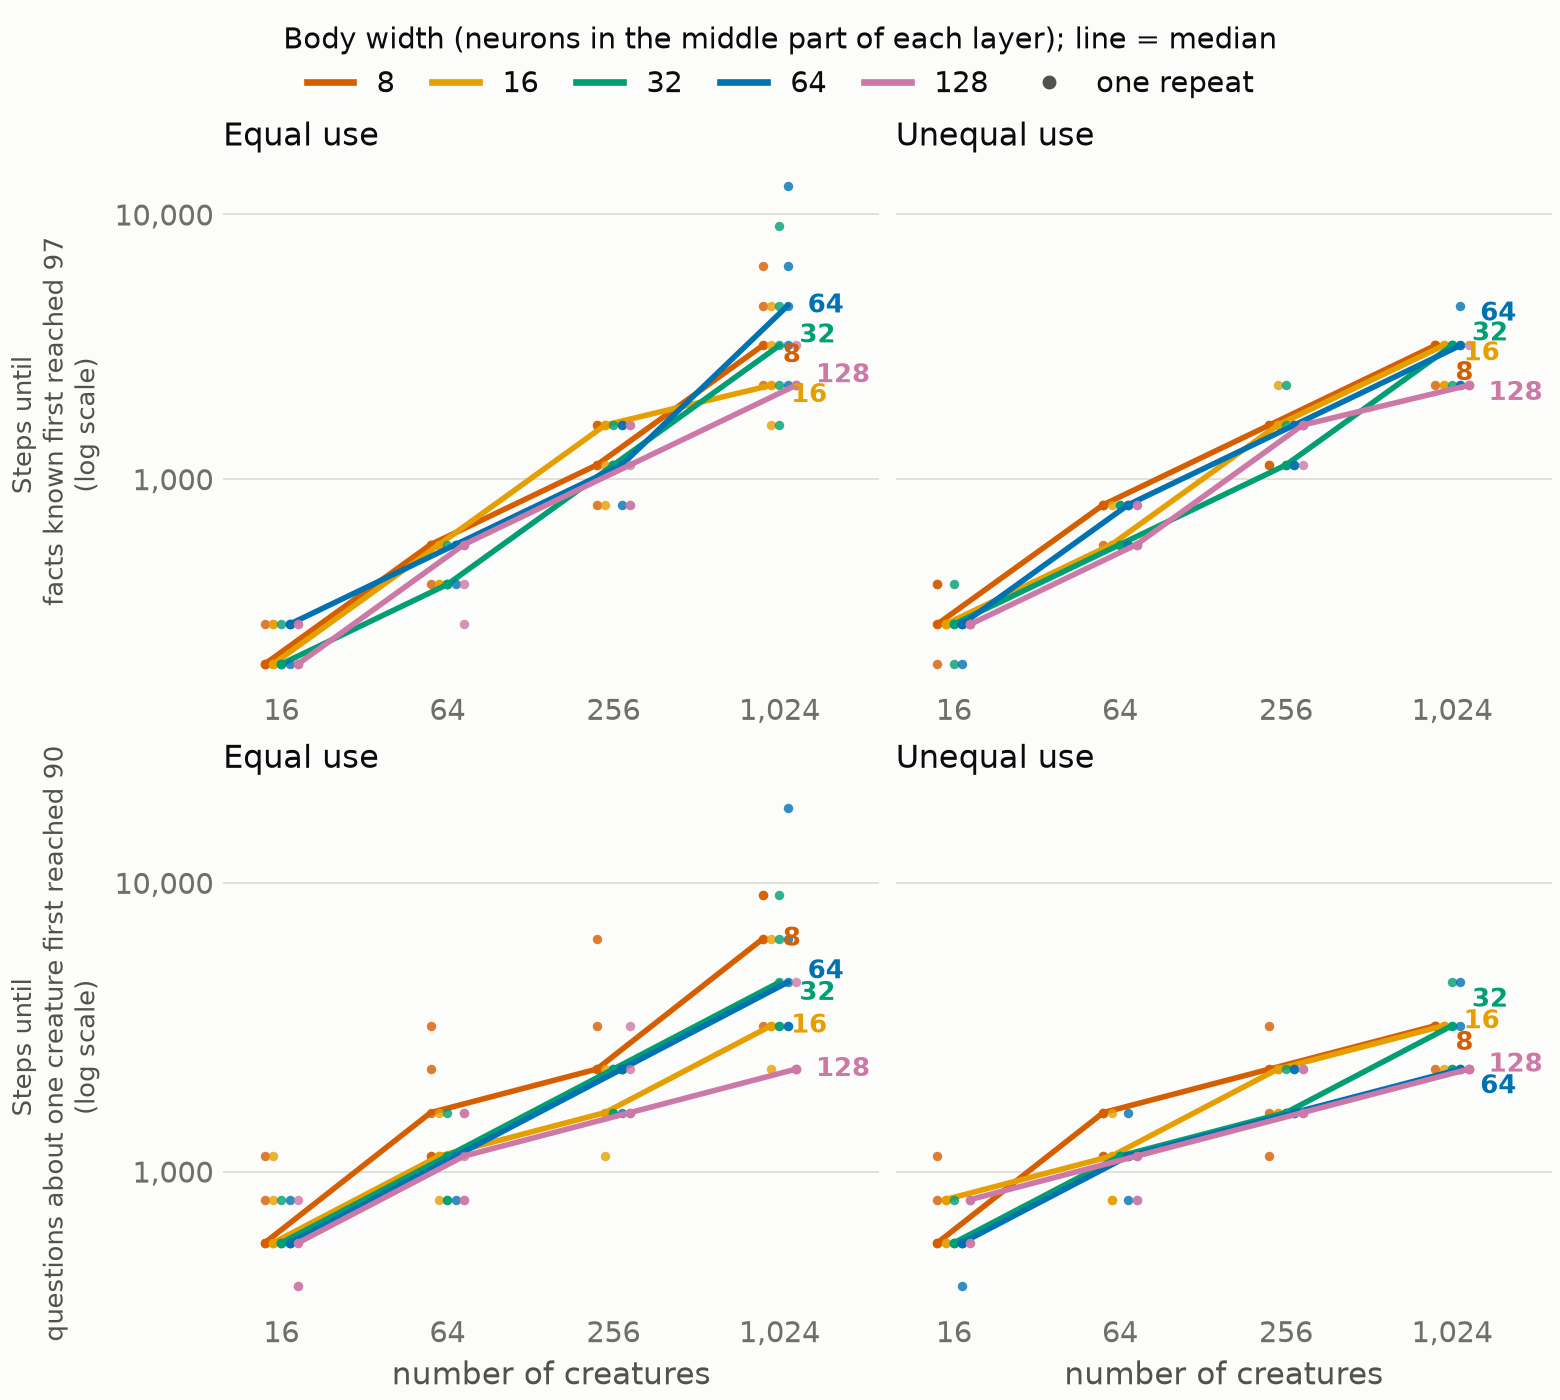
\includegraphics[width=0.62\textwidth]{figures/fig2_speed.png}
\caption{Training steps until the score was first reached, at 8 bits per creature.}\label{fig:speed}
\end{figure}

\reads{fig:speed} Both rows have the number of creatures along the bottom and training steps up
the side, on a scale where each gridline is ten times higher (so a straight line is steady
growth). Top row: the first grading at which facts known was \N{rule.facts_goal} or more. Bottom row:
the first grading at which questions about one creature were \N{rule.questions_goal} or more. A low
dot means learned early. The model was graded at fixed steps, so the values come in jumps. Lines
join the middle of the repeats; the dots are the repeats.

\shows{fig:speed} More creatures took more steps. With equal use, body width 8 needed a median
of \N{main8.c16.b8.equal.steps97.med} steps for the facts at 16 creatures and
\N{main8.c1024.b8.equal.steps97.med} at 1,024; body width 128 needed
\N{main8.c16.b128.equal.steps97.med} and \N{main8.c1024.b128.equal.steps97.med}. For questions
about one creature, body width 8 needed \N{main8.c16.b8.equal.steps90q.med} and
\N{main8.c1024.b8.equal.steps90q.med}, and body width 128 \N{main8.c16.b128.equal.steps90q.med}
and \N{main8.c1024.b128.equal.steps90q.med}. Every run reached both goals. All of this happened in a
small share of the \N{steps.main8} steps trained. The bigger body was a little faster at 1,024
creatures, and the unequal use took a similar number of steps (\N{main8.c1024.b8.zipf.steps97.med} for
the facts at body width 8).

\subsection{The three other scores}

\begin{figure}[H]
\centering
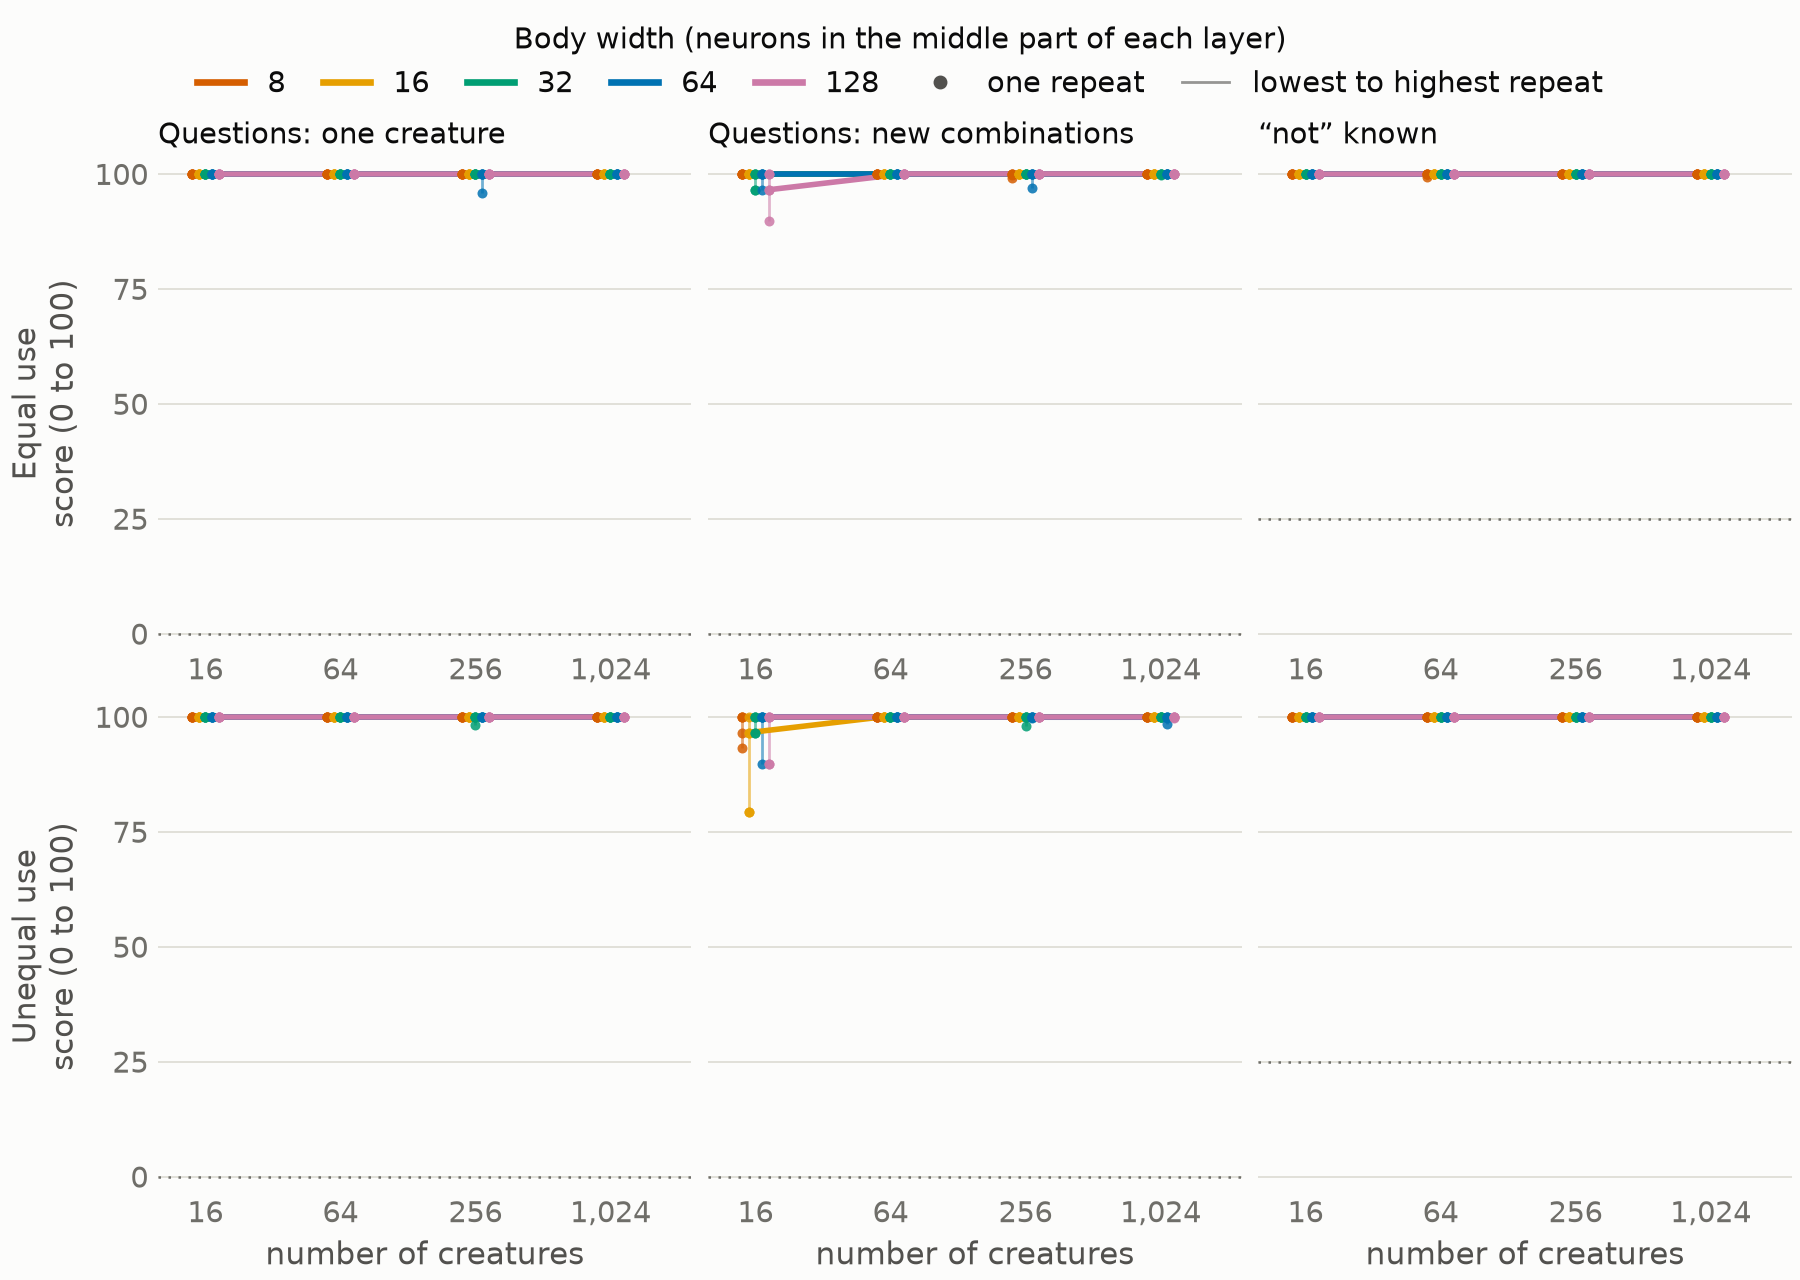
\includegraphics[width=0.8\textwidth]{figures/fig3_questions.png}
\caption{Questions about one creature, questions about new combinations, and ``not'' known, at 8 bits per creature.}\label{fig:others}
\end{figure}

\reads{fig:others} The same layout as figure \ref{fig:main}, one panel for each score. Top row: equal
use. Bottom row: unequal use. Dotted lines mark pure guessing (0 for the two question scores, 25
for ``not'' known).

\shows{fig:others} Almost every dot is on 100 again. The lowest median of any setting was
\N{main8.q1.lowest} for questions about one creature, \N{main8.qnew.lowest} for questions about
new combinations and \N{main8.notk.lowest} for ``not'' known. The few dots below 100 are single
repeats on questions about new combinations, mostly with 16 creatures, where the score rests on
only \N{qnew.count.c16} questions, so one wrong answer moves it. The model could answer about pairs it
had never read together.

\subsection{How the number of trained numbers grows with the vocabulary}

\begin{figure}[H]
\centering
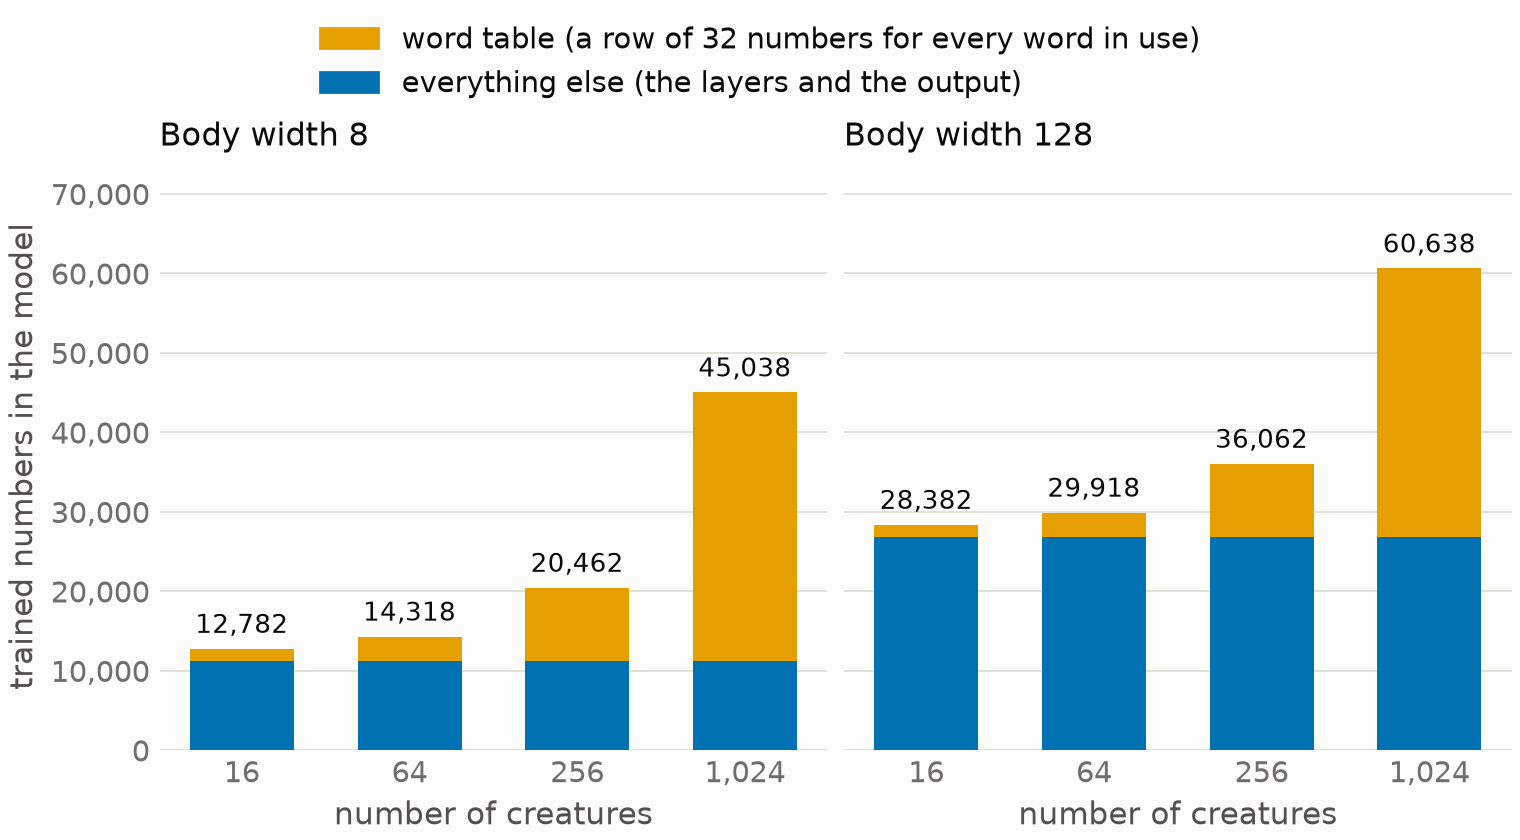
\includegraphics[width=0.68\textwidth]{figures/fig4_parameters.png}
\caption{Trained numbers in the model by number of creatures, for body width 8 and 128.}\label{fig:params}
\end{figure}

\reads{fig:params} Each bar is one model. Its height is the count of trained numbers. Orange is the
word table, which holds a row of \N{rule.columns} numbers for every word in use. Blue is everything
else. The left panel is body width 8, the right one body width 128.

\shows{fig:params} The blue part does not move with the vocabulary: \N{main8.c16.b8.equal.params.rest} for
body width 8 and \N{main8.c16.b128.equal.params.rest} for body width 128. The orange part grows
with every creature. Body width 8 has \N{main8.c16.b8.equal.params.trained} trained numbers with 16
creatures and \N{main8.c1024.b8.equal.params.trained} with 1,024. Body width 128 has
\N{main8.c16.b128.equal.params.trained} and \N{main8.c1024.b128.equal.params.trained}.

\textbf{Why this matters for the claim.} The claim says a vocabulary of a given size strains a model
of a given size. Here the model does not stay the same size when the vocabulary grows: each new
word brings its own row of \N{rule.columns} trained numbers, a place to keep what the model knows about
it. With 1,024 creatures and body width 8 the word table holds \N{main8.c1024.b8.equal.params.table}
of the \N{main8.c1024.b8.equal.params.trained} trained numbers. This report does not show that this
is why the facts were all known. It only shows that the size of the model grew with the
vocabulary, so the test did not hold the model fixed. A frozen table would.

\section{Results at 16, 32 and 64 bits per creature}\label{sec:bits}

No outcome was predicted for these stages, except one sentence in P4: \emph{if anything fails,
the agent expects it to follow the bits per creature and the body width, not the number of
creatures.} The stages below test that sentence. Another way to say how much each number in a
word's row has to hold is bits per creature divided by \N{rule.columns}, the length of a row. It is
0.25 at 8 bits, 0.5 at 16, 1 at 32 and 2 at 64. The pictures print it in brackets.

\begin{center}\small
\begin{tabular}{@{}rrrrrrr@{}}
\toprule
Bits per creature & Kinds of fact & Bits per number & Runs done (of planned) & Repeats & Steps & Learning rate\\
\midrule
8 & 4 & 0.25 & \N{runs.main8} (\N{expected.main8}) & \N{rule.repeats} & \N{steps.main8} & \N{lr.main8}\\
16 & 8 & 0.5 & \N{runs.bits16} (\N{expected.bits16}) & 3 & \N{steps.bits16} & \N{lr.bits16}\\
32 & 16 & 1 & \N{runs.bits32} (\N{expected.bits32}) & 3 & \N{steps.bits32} & \N{lr.bits32}\\
64 & 32 & 2 & \N{runs.bits64} (\N{expected.bits64}) & 2 & \N{steps.bits64} & \N{lr.bits64}\\
\bottomrule
\end{tabular}
\end{center}

\subsection{Facts known}

\begin{figure}[H]
\centering
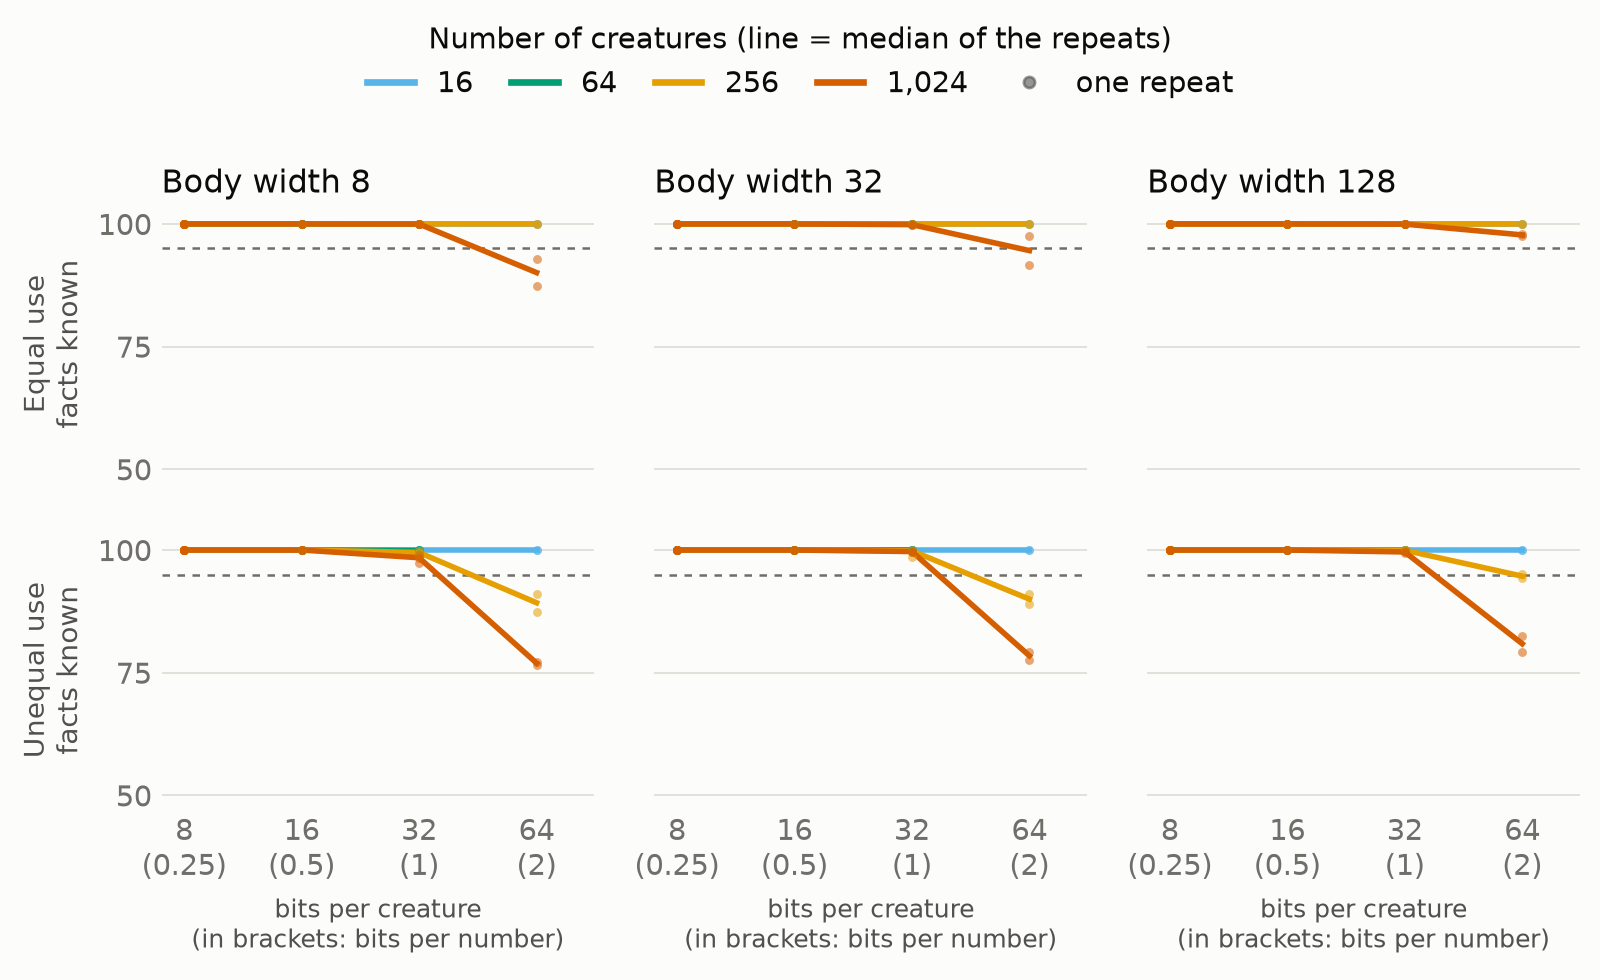
\includegraphics[width=0.62\textwidth]{figures/fig5_bits_facts.png}
\caption{Facts known against bits per creature, for body widths 8, 32 and 128.}\label{fig:bitsfacts}
\end{figure}

\reads{fig:bitsfacts} Along the bottom: bits per creature, with bits per number in brackets. Up the
side: facts known. \textbf{The side starts at 48, not 0,} so the differences can be seen. Each
colour is a number of creatures (the line is the median of the repeats, the dots are the
repeats). Top row: equal use. Bottom row: unequal use. Each column is a body width. At 64 bits there
are no runs with 64 creatures, and the line for 64 creatures is hidden below the others where they
overlap. The dashed line is \N{rule.held}.

\shows{fig:bitsfacts} At 16 bits per creature the lowest median facts known was
\N{bits16.facts.lowest}, so every setting was at the top. At 32 bits it was \N{bits32.facts.lowest}
(\N{bits32.facts.lowest.where}) and the highest \N{bits32.facts.highest}; no setting had a median
below \N{rule.held} (\N{below95.bits32} of \N{settings.bits32}). At 64 bits the medians ran from
\N{bits64.facts.lowest} (\N{bits64.facts.lowest.where}) to \N{bits64.facts.highest}, and
\N{below95.bits64} of \N{settings.bits64} settings ended below \N{rule.held}: \N{below95.bits64.equal} with
equal use and \N{below95.bits64.zipf} with unequal use. Only at 64 bits, and only with many
creatures, did the median facts known fall below \N{rule.held}. With 16 creatures every setting at every stage stayed at
\N{bits64.c16.b8.equal.facts.med} or close to it.

\subsection{The other scores}

\begin{figure}[H]
\centering
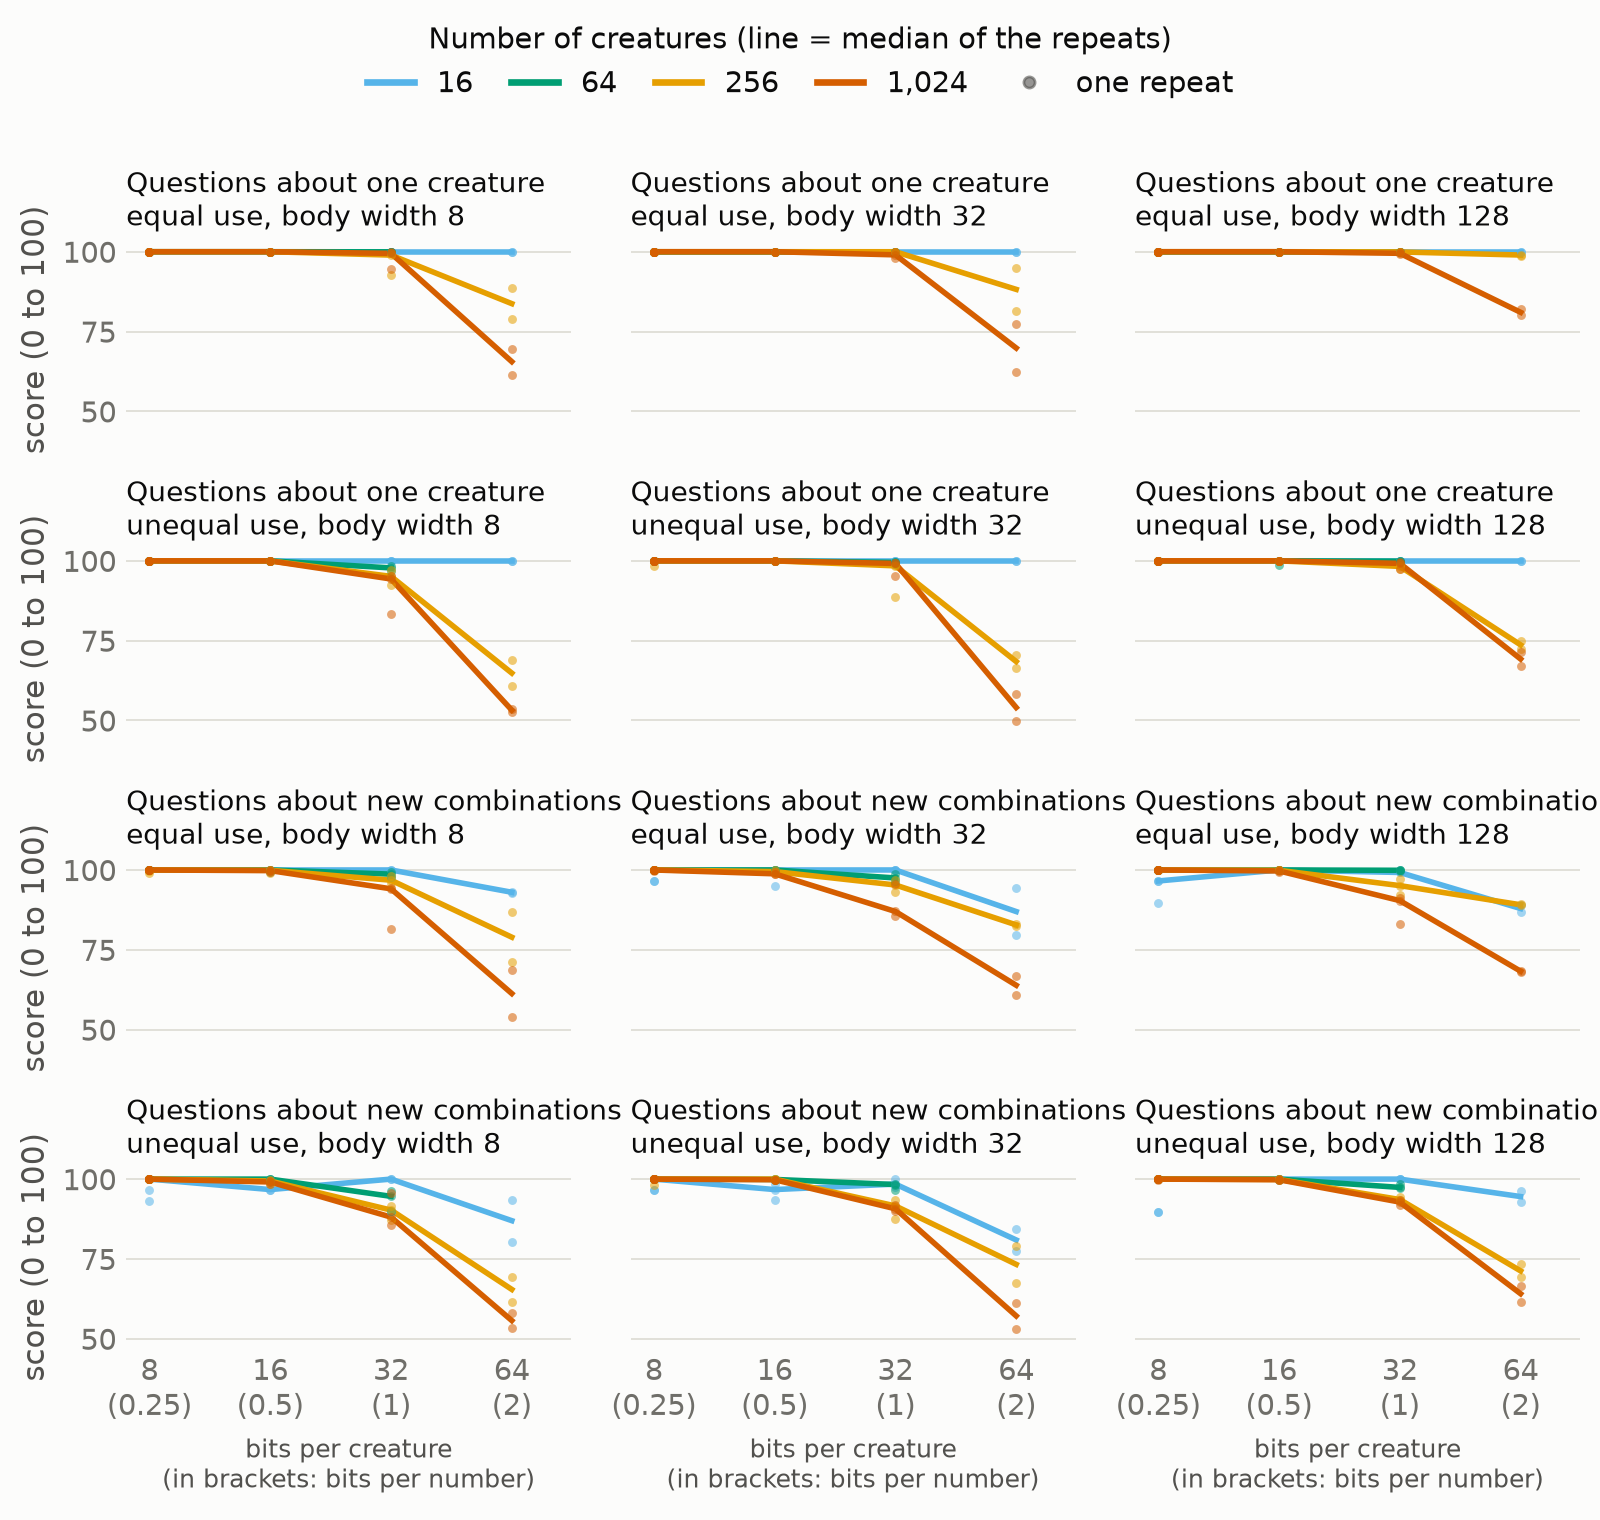
\includegraphics[width=0.6\textwidth]{figures/fig6_bits_questions.png}
\caption{Questions about one creature (top four rows) and about new combinations (bottom four rows) against bits per creature.}\label{fig:bitsq}
\end{figure}

\begin{figure}[H]
\centering
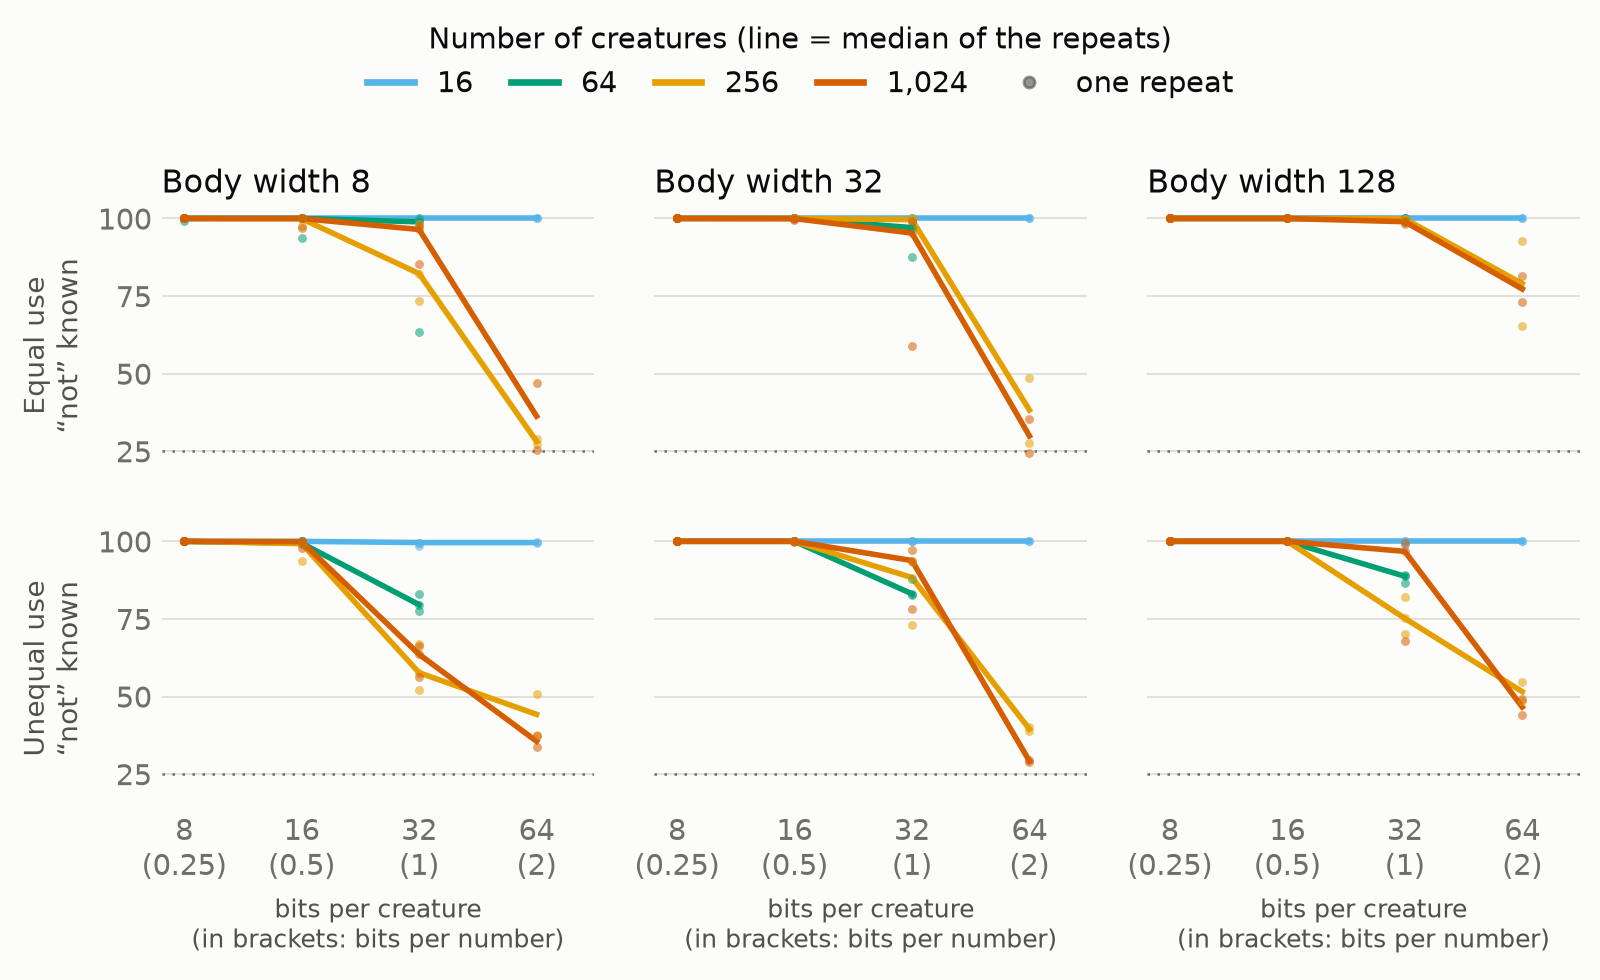
\includegraphics[width=0.62\textwidth]{figures/fig9_bits_notknown.png}
\caption{``not'' known against bits per creature.}\label{fig:bitsnot}
\end{figure}

\reads{fig:bitsq} The same layout as figure \ref{fig:bitsfacts}, but now each panel has its own
title and rows run through the two scores and the two kinds of use. The side starts at 48. In
figure \ref{fig:bitsnot} the side starts at 15 and the dotted line is guessing (25).

\shows{fig:bitsq} The question scores fell sooner and further than facts known. Questions about
one creature: lowest median \N{bits16.q1.lowest} at 16 bits, \N{bits32.q1.lowest} at 32 bits and
\N{bits64.q1.lowest} at 64 bits. Questions about new combinations: \N{bits16.qnew.lowest},
\N{bits32.qnew.lowest} and \N{bits64.qnew.lowest}. The score on new combinations was mostly the same as on combinations the model had read (new minus read: a median
of \N{qdiff.median} points over all settings, and never below \N{qdiff.others.lowest}
anywhere except with 16 creatures at 64 bits). There it went down to \N{qdiff.bits64.c16.lowest}
points, on very few questions (\N{qnew.count.c16}), so it may be chance. \textbf{``not'' known} (figure \ref{fig:bitsnot}) fell the furthest: lowest median
\N{bits16.notk.lowest} at 16 bits, \N{bits32.notk.lowest} at 32 bits and \N{bits64.notk.lowest}
at 64 bits, which is near guessing (25). With 16 creatures it stayed at \N{notk.c16.lowest} or more in every stage.

\subsection{Which settings were still rising? (64 bits)}

\begin{figure}[H]
\centering
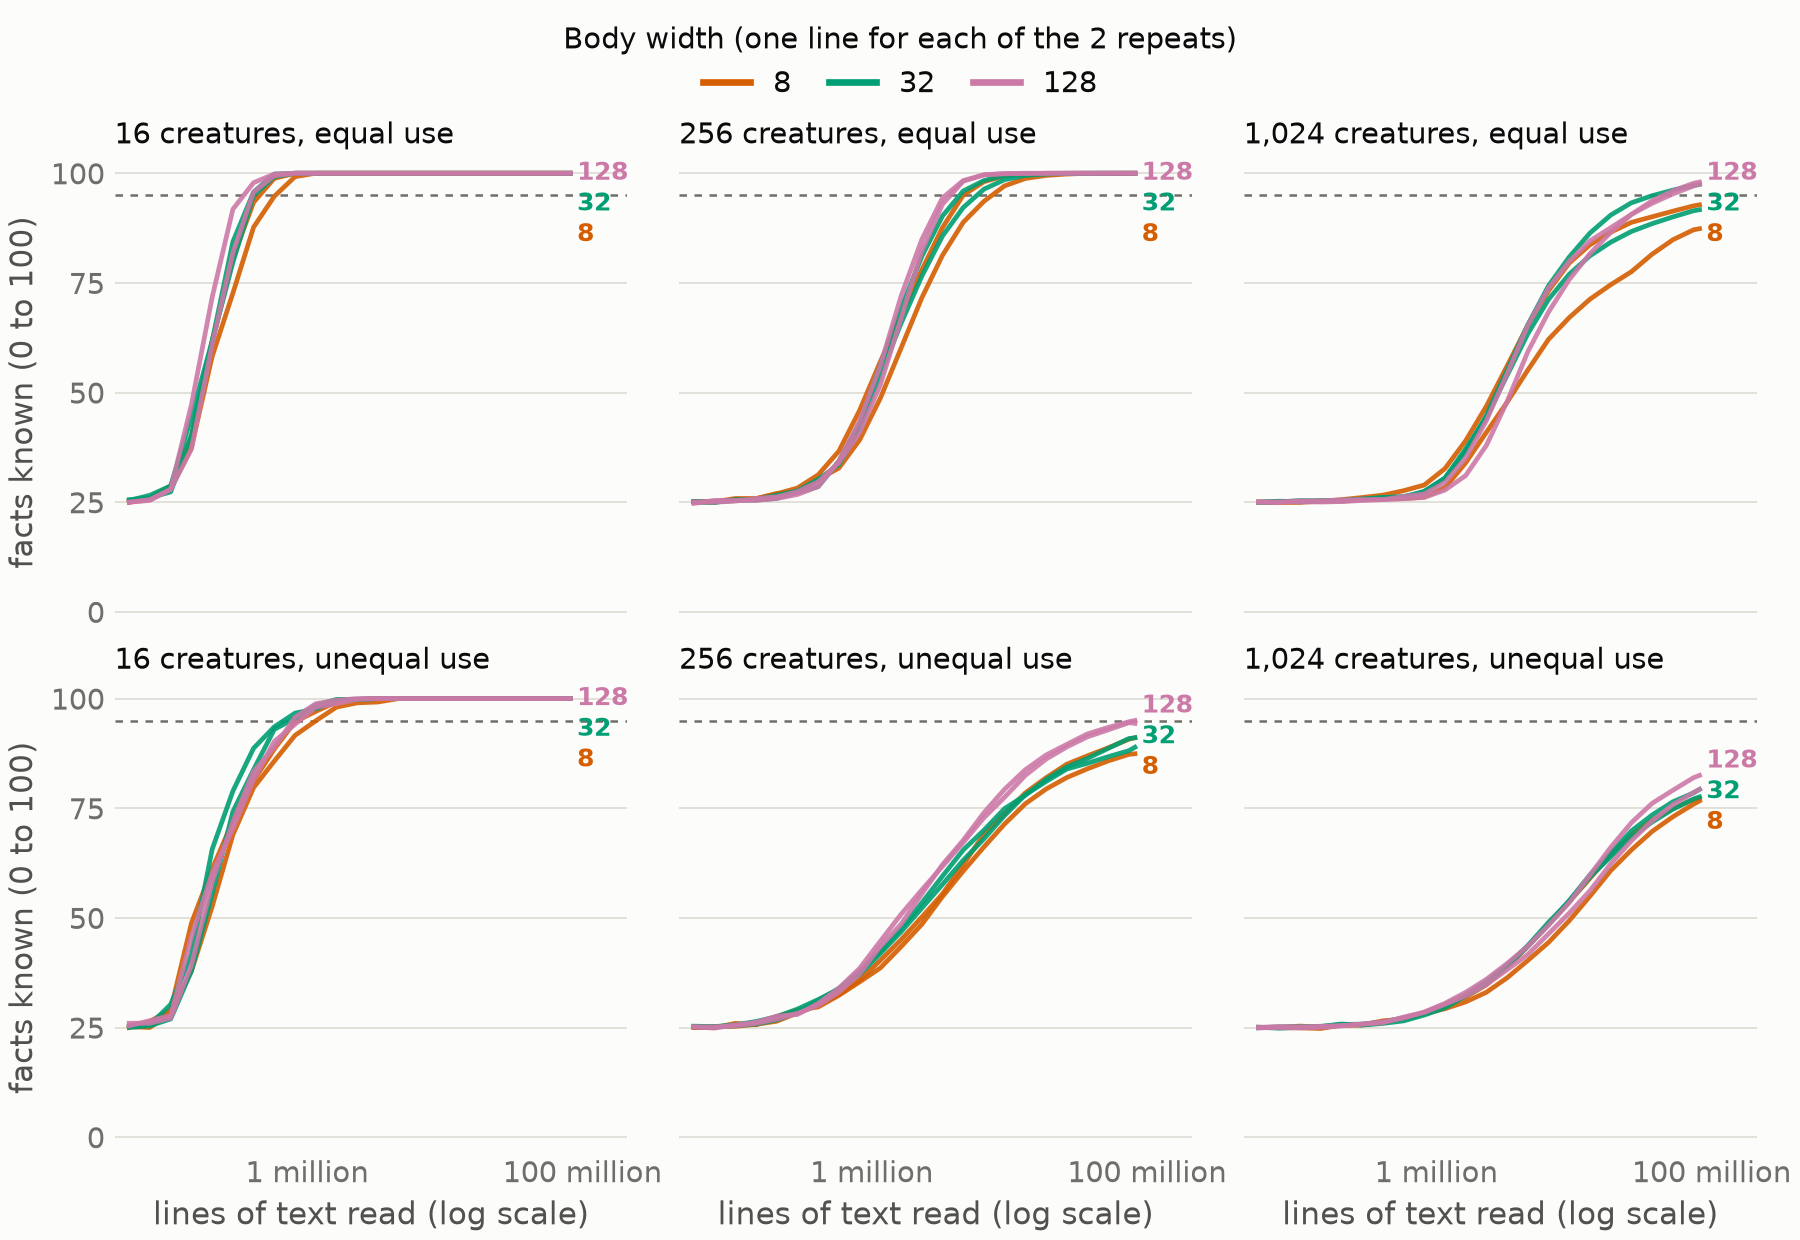
\includegraphics[width=0.7\textwidth]{figures/fig7_curves64.png}
\caption{Learning curves at 64 bits per creature: facts known against lines of text read.}\label{fig:curves}
\end{figure}

\reads{fig:curves} Each line is one run. Along the bottom: how many lines of text the model had read,
on a scale where each tick is a hundred times the one before. Up the side: facts known. The
columns are 16, 256 and 1,024 creatures, the rows are equal and unequal use. Colour is the body
width. The dashed line is \N{rule.held}.

\shows{fig:curves} With 16 and, for equal use, 256 creatures, the curves reach the top and
stay there. For the other settings the lines are still climbing at the right edge, where training
stopped. A setting counts as \emph{still rising} if its median gained at least \N{rule.rise} point in the
second half of training. Of the \N{below95.bits64} settings below \N{rule.held} at 64 bits,
\N{below95.rising.bits64} were still rising and \N{below95.flat.bits64} were not. No setting at 8, 16
or 32 bits ended below \N{rule.held} (\N{below95.main8}, \N{below95.bits16} and \N{below95.bits32}).
\textbf{So for every low score at 64 bits, this report cannot tell ``cannot hold'' from ``not
learned yet''}: the longer control run, which would have told them apart, was not done.

\paragraph{64 bits per creature.} 8 settings ended with a median below 95.

\begin{center}\small
\begin{tabular}{@{}llrrrrl@{}}
\toprule
Word use & Creatures & Body width & Median & Lowest to highest & Gain in the second half & Still rising?\\
\midrule
Equal use & 1,024 & 8 & 90.1 & 87.4 to 92.8 & +4.3 & yes\\
Equal use & 1,024 & 32 & 94.6 & 91.7 to 97.5 & +2.9 & yes\\
Unequal use & 256 & 8 & 89.2 & 87.4 to 91.1 & +3.8 & yes\\
Unequal use & 256 & 32 & 90.0 & 88.9 to 91.1 & +4.2 & yes\\
Unequal use & 256 & 128 & 94.7 & 94.3 to 95.0 & +3.1 & yes\\
Unequal use & 1,024 & 8 & 77.0 & 76.7 to 77.2 & +5.9 & yes\\
Unequal use & 1,024 & 32 & 78.4 & 77.6 to 79.3 & +5.8 & yes\\
Unequal use & 1,024 & 128 & 80.9 & 79.3 to 82.5 & +6.8 & yes\\
\bottomrule
\end{tabular}
\end{center}


\subsection{Testing the sentence in P4}

Table below gives, for every stage and kind of use, how much the score on facts known fell from
16 to 1,024 creatures at three body widths (a positive number means 1,024 creatures scored
lower), and how much it rose from body width 8 to 128 with 1,024 creatures. Medians.

\begin{center}\small
\begin{tabular}{@{}llrrrr@{}}
\toprule
 & & \multicolumn{3}{c}{Fall from 16 to 1,024 creatures} & Rise from body 8 to 128\\
Bits per creature & Use & at body 8 & at body 32 & at body 128 & at 1,024 creatures\\
\midrule
8 & equal & \N{gap.creatures.main8.equal.b8} & \N{gap.creatures.main8.equal.b32} & \N{gap.creatures.main8.equal.b128} & \N{gap.body.main8.equal.c1024}\\
8 & unequal & \N{gap.creatures.main8.zipf.b8} & \N{gap.creatures.main8.zipf.b32} & \N{gap.creatures.main8.zipf.b128} & \N{gap.body.main8.zipf.c1024}\\
16 & equal & \N{gap.creatures.bits16.equal.b8} & \N{gap.creatures.bits16.equal.b32} & \N{gap.creatures.bits16.equal.b128} & \N{gap.body.bits16.equal.c1024}\\
16 & unequal & \N{gap.creatures.bits16.zipf.b8} & \N{gap.creatures.bits16.zipf.b32} & \N{gap.creatures.bits16.zipf.b128} & \N{gap.body.bits16.zipf.c1024}\\
32 & equal & \N{gap.creatures.bits32.equal.b8} & \N{gap.creatures.bits32.equal.b32} & \N{gap.creatures.bits32.equal.b128} & \N{gap.body.bits32.equal.c1024}\\
32 & unequal & \N{gap.creatures.bits32.zipf.b8} & \N{gap.creatures.bits32.zipf.b32} & \N{gap.creatures.bits32.zipf.b128} & \N{gap.body.bits32.zipf.c1024}\\
64 & equal & \N{gap.creatures.bits64.equal.b8} & \N{gap.creatures.bits64.equal.b32} & \N{gap.creatures.bits64.equal.b128} & \N{gap.body.bits64.equal.c1024}\\
64 & unequal & \N{gap.creatures.bits64.zipf.b8} & \N{gap.creatures.bits64.zipf.b32} & \N{gap.creatures.bits64.zipf.b128} & \N{gap.body.bits64.zipf.c1024}\\
\bottomrule
\end{tabular}
\end{center}

\textbf{The expectation was wrong at 64 bits.} It said that failure would follow the bits per
creature and the body width, not the number of creatures. At 64 bits, larger vocabularies did score
lower at every body width, with both kinds of use. With equal use the fall was \N{gap.creatures.bits64.equal.b8}
points at body width 8, \N{gap.creatures.bits64.equal.b32} at 32 and
\N{gap.creatures.bits64.equal.b128} at 128. With unequal use it was \N{gap.creatures.bits64.zipf.b8},
\N{gap.creatures.bits64.zipf.b32} and \N{gap.creatures.bits64.zipf.b128}. The fall was at least
\N{rule.gap} points in \N{gap.creatures.big.bits64.zipf} of \N{gap.creatures.n.bits64.zipf} body
widths with unequal use and in \N{gap.creatures.big.bits64.equal} of \N{gap.creatures.n.bits64.equal} with equal use. The bits mattered too: with
16 creatures nothing fell at 64 bits (facts known stayed at \N{bits64.c16.b8.equal.facts.med}), so
bits alone did not cause the fall. The score fell with the number of creatures \emph{and} the
bits together. At 16 and 32 bits, with the facts as the score, the number of creatures made almost no
difference (a fall of \N{gap.creatures.bits16.equal.b8} to \N{gap.creatures.bits32.zipf.b16} points),
so there the expectation held. A bigger body helped a little at 64 bits (a rise of
\N{gap.body.bits64.equal.c1024} points with equal use, \N{gap.body.bits64.zipf.c1024} with unequal use),
less than the fall caused by more creatures.

\textbf{Equal and unequal use compared.} Equal use was never worse than unequal use at the same
stage and body width. At 64 bits and 1,024 creatures the median facts known at body width 8 was
\N{bits64.c1024.b8.equal.facts.med} with equal use and \N{bits64.c1024.b8.zipf.facts.med} with unequal
use. With unequal use the rarest creatures are read far less often than the others, so some of the
unequal-use fall may be learning that has not got round to them yet. This was not tested.

\textbf{A caution about the total number of bits.} 1,024 creatures at 16 bits and 256 creatures at
64 bits both hold the same total number of bits. With unequal use and body width 8 the first stood at
\N{bits16.c1024.b8.zipf.facts.med} facts known and the second at \N{bits64.c256.b8.zipf.facts.med}. With
equal use the two were \N{bits16.c1024.b8.equal.facts.med} and \N{bits64.c256.b8.equal.facts.med}. So
the total number of bits did not line up the results by itself. Only two points are compared here, and the
64-bit runs also used a different learning rate and length.

